%
%                  Politecnico di Milano
%
%         Student: Caravano Andrea, Alberto Cantele
%            A.Y.: 2024/2025
%
%   Last modified: 20/05/2025
%
%     Description: Internet of Things: Homework
%                  Exercise n. 3
%

\documentclass[a4paper,11pt]{article} % tipo di documento
\usepackage[T1]{fontenc} % codifica dei font
\usepackage[utf8]{inputenc} % lettere accentate da tastiera
\usepackage[english]{babel} % lingua del documento
\usepackage{lipsum} % genera testo fittizio
\usepackage{url} % per scrivere gli indirizzi Internet e/o di riferimento nella pagina

\usepackage{hyperref} % per modificare il comportamento dei collegamenti ipertestuali

\usepackage[margin=0.7in]{geometry} % margine di pagina

\usepackage{graphicx} % per inserire immagini

\usepackage{minted} % per colorazione automatica del codice (installare pygments da Homebrew)
% \usepackage{pythonhighlight} % per Python

\setminted{ % si può impostare il linguaggio specifico con \setminted[JSON] ad esempio
    linenos=true,
    breaklines=true,
    encoding=utf8,
    fontsize=\normalsize,
    frame=lines
}

\usepackage{fancyhdr}
\usepackage{textcomp}
\usepackage{siunitx} % per gestione intestazione e piè di pagina

\usepackage{tcolorbox} % per riquadrature di vario colore

\usepackage{float} % per figure comparative flottanti
\usepackage[fleqn]{amsmath} % per frazioni in display style e sistemi di equazioni, allineate a sinistra

\usepackage{icomma} % virgola come separatore decimale

\usepackage{titlesec} % per configurazione del tipo paragrafo

\usepackage{multirow} % righe multiple in tabelle

\usepackage{subfig} % descrizione sottostante a figure

% setup del tipo paragrafo
\setcounter{secnumdepth}{4}

\titleformat{\paragraph}
{\normalfont\normalsize\bfseries}{\theparagraph}{1em}{}
\titlespacing*{\paragraph}
{0pt}{3.25ex plus 1ex minus .2ex}{1.5ex plus .2ex}

\hypersetup{ % metadati di titolo e autore nel PDF
    hidelinks, % leva colore attorno collegamenti ipertestuali
    pdftitle={Internet of Things: Homework - exercise n. 3},
    pdfauthor={Andrea Caravano, Alberto Cantele}
}

\setlength{\parindent}{0pt} % rimuove l'indentazione del testo

\tcbset{ % impostazioni per riquadrature
    colback=gray!20,
    colframe=black,
    boxrule=0.5pt
}

\captionsetup{labelformat=empty} % rimuove la caption delle figure

% Imposta la profondità dell'indice a 2 livelli (sottosezioni, non sotto-sottosezioni)
\setcounter{tocdepth}{2}

\pagestyle{fancy}
\fancyhead{}\fancyfoot{}
\fancyhead[L]{\textbf{Internet of Things: Homework - exercise n. 3}}
\fancyhead[R]{Andrea Caravano, Alberto Cantele}
\fancyfoot[C]{\thepage}

\title{\textbf{Internet of Things}\\Homework: exercise n. 3}
\author{Andrea Caravano, Alberto Cantele}
\date{Academic Year 2024--25}

\begin{document}
\maketitle

%\tableofcontents

\section*{Exercise text}
A RFID system based on Dynamic Frame ALOHA is composed of $N=4$ tags

\begin{enumerate}
    \item Find the overall collision resolution efficiency $\eta$ in the different cases in which the initial frame size is set to $r_1$ = 1, 2, 3, 4, 5, 6.
        \begin{itemize}
            \item Assume that after the first frame, the frame size is correctly set to the current backlog size.
            \item Assume as given the duration of the arbitration period with $N$ = 2, 3 tags when $r = N$ ($L_2 = 4$, $L_3 = \dfrac{51}{8}$).
        \end{itemize}
    \item After computing the values of the efficiency with the different frame sizes, produce a plot with values of $\eta$ over $r_1$.
    \item For what values of $r_1$ we have the maximum value for $\eta$? Comment.
\end{enumerate}

\section{Collision resolution efficiency}

Given, as computed during the exercise lectures,

\smallskip

$L_2 = 4$

\medskip

$L_3 = \dfrac{51}{8}$

\medskip

And adding, trivially,

\smallskip

$L_1 = 1$

\medskip

We are now aiming at computing the missing $L_4$, which will be useful in the successive steps of the computation, which will in fact make use of the backlog size.

% Resetta il contatore delle sotto-sottosezioni a -1
\setcounter{subsection}{-1}

\subsection{The missing piece: $L_4$}\label{computation-L4}

Being the frame size ($r$) equal to the number of tags ($N$), $r = N$, the generic recursive formula applies:

\smallskip

$L_4 = 4 + \displaystyle\sum_{i = 0}^{3} L_{4-i} \cdot P(S = i)$

\smallskip

With $S$ be the number of resolved tags.

\medskip

The overall resolutive strategies then outlines the classic probabilistic characteristics of the problem by exploiting $\dfrac{Matching\ cases}{Possible\ cases}$, combining and permuting them in the classic slot allocation fashion.

\smallskip

The term accounting for possible cases, $\left(\dfrac{1}{r}\right)^N$, will, in fact, always be present.

\medskip

$P(S = 0) = \left(\dfrac{1}{4}\right)^4 \cdot \left(4 + \displaystyle\binom{4}{2} \cdot \dfrac{4!}{2 \cdot 2}\right) = \dfrac{10}{64}$, which accounts for the cases in which all the tags collide or the cases for which they collide in pairs (groups of 2), being the only possible one leading to no resolved tag.

\medskip

$P(S = 1) = \left(\dfrac{1}{4}\right)^4 \cdot 4 \cdot 4 \cdot 3 = \dfrac{3}{16}$, which accounts for the number of tags to solve, the ways of solving them and the ways of positioning the remaining ones.

\medskip

$P(S = 2) = \left(\dfrac{1}{4}\right)^4 \cdot \displaystyle \binom{4}{2} \cdot 4! = \dfrac{9}{16}$, which again considers the case in which pairs of tag collide.

\medskip

$P(S = 3) = 0$, being impossible solving 3 tags over 4: the remaining tag would be either collided with another one or solved itself.

\medskip

$P(S = 4) = \left(\dfrac{1}{4}\right)^4 \cdot 4! = \dfrac{6}{64}$, which accounts for the possible permutations of the 4 solved tags.

\medskip

Which ultimately sums up to 1, as expected by enumerating all possible cases.

\bigskip

The overall result will therefore be:

\medskip

$L_4 = 4 + \dfrac{10}{64} \cdot L_4 + \dfrac{3}{16} \cdot L_3 + \dfrac{9}{16} \cdot L_2 = 4 + \dfrac{10}{64} L_4 + \dfrac{3}{16} \cdot \dfrac{51}{8} + \dfrac{9}{16} \cdot 4 = \dfrac{953}{108} = 8,824$.

\subsection{Case $r_1 = 1$}

All tags will trivially collide in the only available slot, which translates to:

\smallskip

$P(S = 0) = 1$

\smallskip

$P(S = 1) = P(S = 2) = P(S = 3) = P(S = 4) = 0$

\bigskip

Which ultimately leads to:

\medskip

$L^{*} = r_1 + P(S = 0) \cdot L_4 = 1 + 1 \cdot 8,824 = 9,824$

\medskip

$\eta = \dfrac{N}{L^{*}} = \dfrac{4}{9,824} = 0,407$

\subsection{Case $r_1 = 2$}

The maximum number of tags that can be solved in 2 slots is expected to be, intuitively, equal to 1: \hyperref[computation-L4]{as similarly commented earlier}, the remaining tags would either collide or not be present at all.

\medskip

$P(S = 0) = \left(\dfrac{1}{2}\right)^4 \cdot \left(2 + \displaystyle\binom{4}{2}\right) = \dfrac{1}{2}$, which accounts for the cases in which all the tags collide or the cases for which they collide in pairs (groups of 2), being the only possible one leading to no resolved tag.

\medskip

$P(S = 1) = \left(\dfrac{1}{2}\right)^4 \cdot 4 \cdot 2 \cdot 1 = \dfrac{1}{2}$, which accounts for the number of tags to solve, the ways of solving them and the ways of positioning the remaining ones.

\medskip

$P(S = 2) = P(S = 3) = P(S = 4) = 0$, as expected.

\medskip

Which ultimately sums up to 1, as expected by enumerating all possible cases.

\bigskip

The overall result will therefore be:

\medskip

$L^{*} = r_1 + P(S = 0) \cdot L_4 + P(S = 1) \cdot L_3 = 2 + \dfrac{1}{2} \cdot 8,824 + \dfrac{1}{2} \cdot \dfrac{51}{8} = 9,600$

\medskip

$\eta = \dfrac{N}{L^{*}} = \dfrac{4}{9,600} = 0,417$

\subsection{Case $r_1 = 3$}

The maximum number of tags that can be solved in 3 slots is expected to be, intuitively, equal to 2: \hyperref[computation-L4]{as similarly commented earlier}, the remaining tags would either collide or not be present at all.

\medskip

$P(S = 0) = \left(\dfrac{1}{3}\right)^4 \cdot \left(3 + \displaystyle\binom{4}{2} \cdot \dfrac{3!}{2}\right) = \dfrac{7}{27}$, which accounts for the cases in which all the tags collide or the cases for which they collide in pairs (groups of 2), being the only possible one leading to no resolved tag: in such a case, simmetry is also accounted for.

\medskip

$P(S = 1) = \left(\dfrac{1}{3}\right)^4 \cdot 4 \cdot 3 \cdot 2 \cdot 1 = \dfrac{8}{27}$, which accounts for the number of tags to solve, the ways of solving them and the ways of positioning the remaining ones.

\medskip

$P(S = 2) = \left(\dfrac{1}{3}\right)^4 \cdot \displaystyle\binom{4}{2} \cdot 3 \cdot 2 \cdot 1 = \dfrac{4}{9}$, which again considers the case in which pairs of tag collide.

\medskip

$P(S = 3) = P(S = 4) = 0$, as expected.

\medskip

Which ultimately sums up to 1, as expected by enumerating all possible cases.

\bigskip

The overall result will therefore be:

\medskip

$L^{*} = r_1 + P(S = 0) \cdot L_4 + P(S = 1) \cdot L_3 + P(S = 2) \cdot L_2 = 3 + \dfrac{7}{27} \cdot 8,824 + \dfrac{8}{27} \cdot \dfrac{51}{8} + \dfrac{4}{9} \cdot 4 = 8,954$

\medskip

$\eta = \dfrac{N}{L^{*}} = \dfrac{4}{8,954} = 0,447$

\subsection{Case $r_1 = 4$}

Being $r = N$, \hyperref[computation-L4]{as mentioned earlier, the recursive formula described at the beginning} applies.

\smallskip

Therefore, $L^{*} = L_4 = 8,824$

\medskip

$\eta = \dfrac{N}{L^{*}} = \dfrac{4}{8,824} = 0,453$

\subsection{Case $r_1 = 5$}

This time, we will need to consider all cases up to solving all tags, being all theoretically valid.

\medskip

$P(S = 0) = \left(\dfrac{1}{5}\right)^4 \cdot \left(5 + \displaystyle\binom{4}{2} \cdot \dfrac{5 \cdot 4}{2}\right) = \dfrac{13}{125}$, which accounts for the cases in which all the tags collide or the cases for which they collide in pairs (groups of 2), being the only possible one leading to no resolved tag: in such a case, simmetry is also accounted for.

\medskip

$P(S = 1) = \left(\dfrac{1}{5}\right)^4 \cdot 5 \cdot 4 \cdot 4 = \dfrac{16}{125}$, which accounts for the number of tags to solve, the ways of solving them and the ways of positioning the remaining ones.

\medskip

$P(S = 2) = \left(\dfrac{1}{5}\right)^4 \cdot \displaystyle\binom{4}{2} \cdot \dfrac{5 \cdot 4 \cdot 3 \cdot 2 \cdot 1}{2} = \dfrac{72}{125}$, which again considers the case in which pairs of tag collide and accounts for simmetry.

\medskip

$P(S = 3) = 0$, being impossible solving 3 tags over 4: the remaining tag would be either collided with another one or solved itself.

\medskip

$P(S = 4) = \left(\dfrac{1}{5}\right)^4 \cdot 5 \cdot 4 \cdot 3 \cdot 2 \cdot 1 = \dfrac{24}{125}$, which accounts for the possible permutations of the 4 solved tags.

\medskip

Which ultimately sums up to 1, as expected by enumerating all possible cases.

\bigskip

The overall result will therefore be:

\medskip

$L^{*} = r_1 + P(S = 0) \cdot L_4 + P(S = 1) \cdot L_3 + P(S = 2) \cdot L_2 = 5 + \dfrac{13}{125} \cdot 8,824 + \dfrac{16}{125} \cdot \dfrac{51}{8} + \dfrac{72}{125} \cdot 4 = 9,038$

\medskip

$\eta = \dfrac{N}{L^{*}} = \dfrac{4}{9,038} = 0,443$

\subsection{Case $r_1 = 6$}

This last time, again, we will need to consider all cases up to solving all tags, being all theoretically valid.

\medskip

$P(S = 0) = \left(\dfrac{1}{6}\right)^4 \cdot \left(6 + \displaystyle \binom{4}{2} \cdot \dfrac{6 \cdot 5}{2}\right) = \dfrac{2}{27}$, which accounts for the cases in which all the tags collide or the cases for which they collide in pairs (groups of 2), being the only possible one leading to no resolved tag: in such a case, simmetry is also accounted for.

\medskip

$P(S = 1) = \left(\dfrac{1}{6}\right)^4 \cdot 6 \cdot 5 \cdot 4 = \dfrac{5}{54}$, which accounts for the number of tags to solve, the ways of solving them and the ways of positioning the remaining ones.

\medskip

$P(S = 2) = \left(\dfrac{1}{6}\right)^4 \cdot \dfrac{6 \cdot 5 \cdot 4 \cdot 4 \cdot 3}{2} = \dfrac{5}{9}$, which again considers the case in which pairs of tag collide and accounts for simmetry.

\medskip

$P(S = 3) = 0$, being impossible solving 3 tags over 4: the remaining tag would be either collided with another one or solved itself.

\medskip

$P(S = 4) = \left(\dfrac{1}{6}\right)^4 \cdot \displaystyle\binom{6}{2} \cdot 4 \cdot 3 \cdot 2 \cdot 1 = \dfrac{5}{18}$, which accounts for the possible permutations of the 4 solved tags and combinations of the remaining pairs of frame slots.

\medskip

Which ultimately sums up to 1, as expected by enumerating all possible cases.

\bigskip

The overall result will therefore be:

\medskip

$L^{*} = r_1 + P(S = 0) \cdot L_4 + P(S = 1) \cdot L_3 + P(S = 2) \cdot L_2 = 6 + \dfrac{2}{27} \cdot 8,824 + \dfrac{5}{54} \cdot \dfrac{51}{8} + \dfrac{5}{9} \cdot 4 = 9,466$

\medskip

$\eta = \dfrac{N}{L^{*}} = \dfrac{4}{9,466} = 0,423$

\section{Efficiency plot}

The collective efficiency plot is then produced using standard \textsc{Python} libraries, with the result being shown in the following.

\begin{center}
    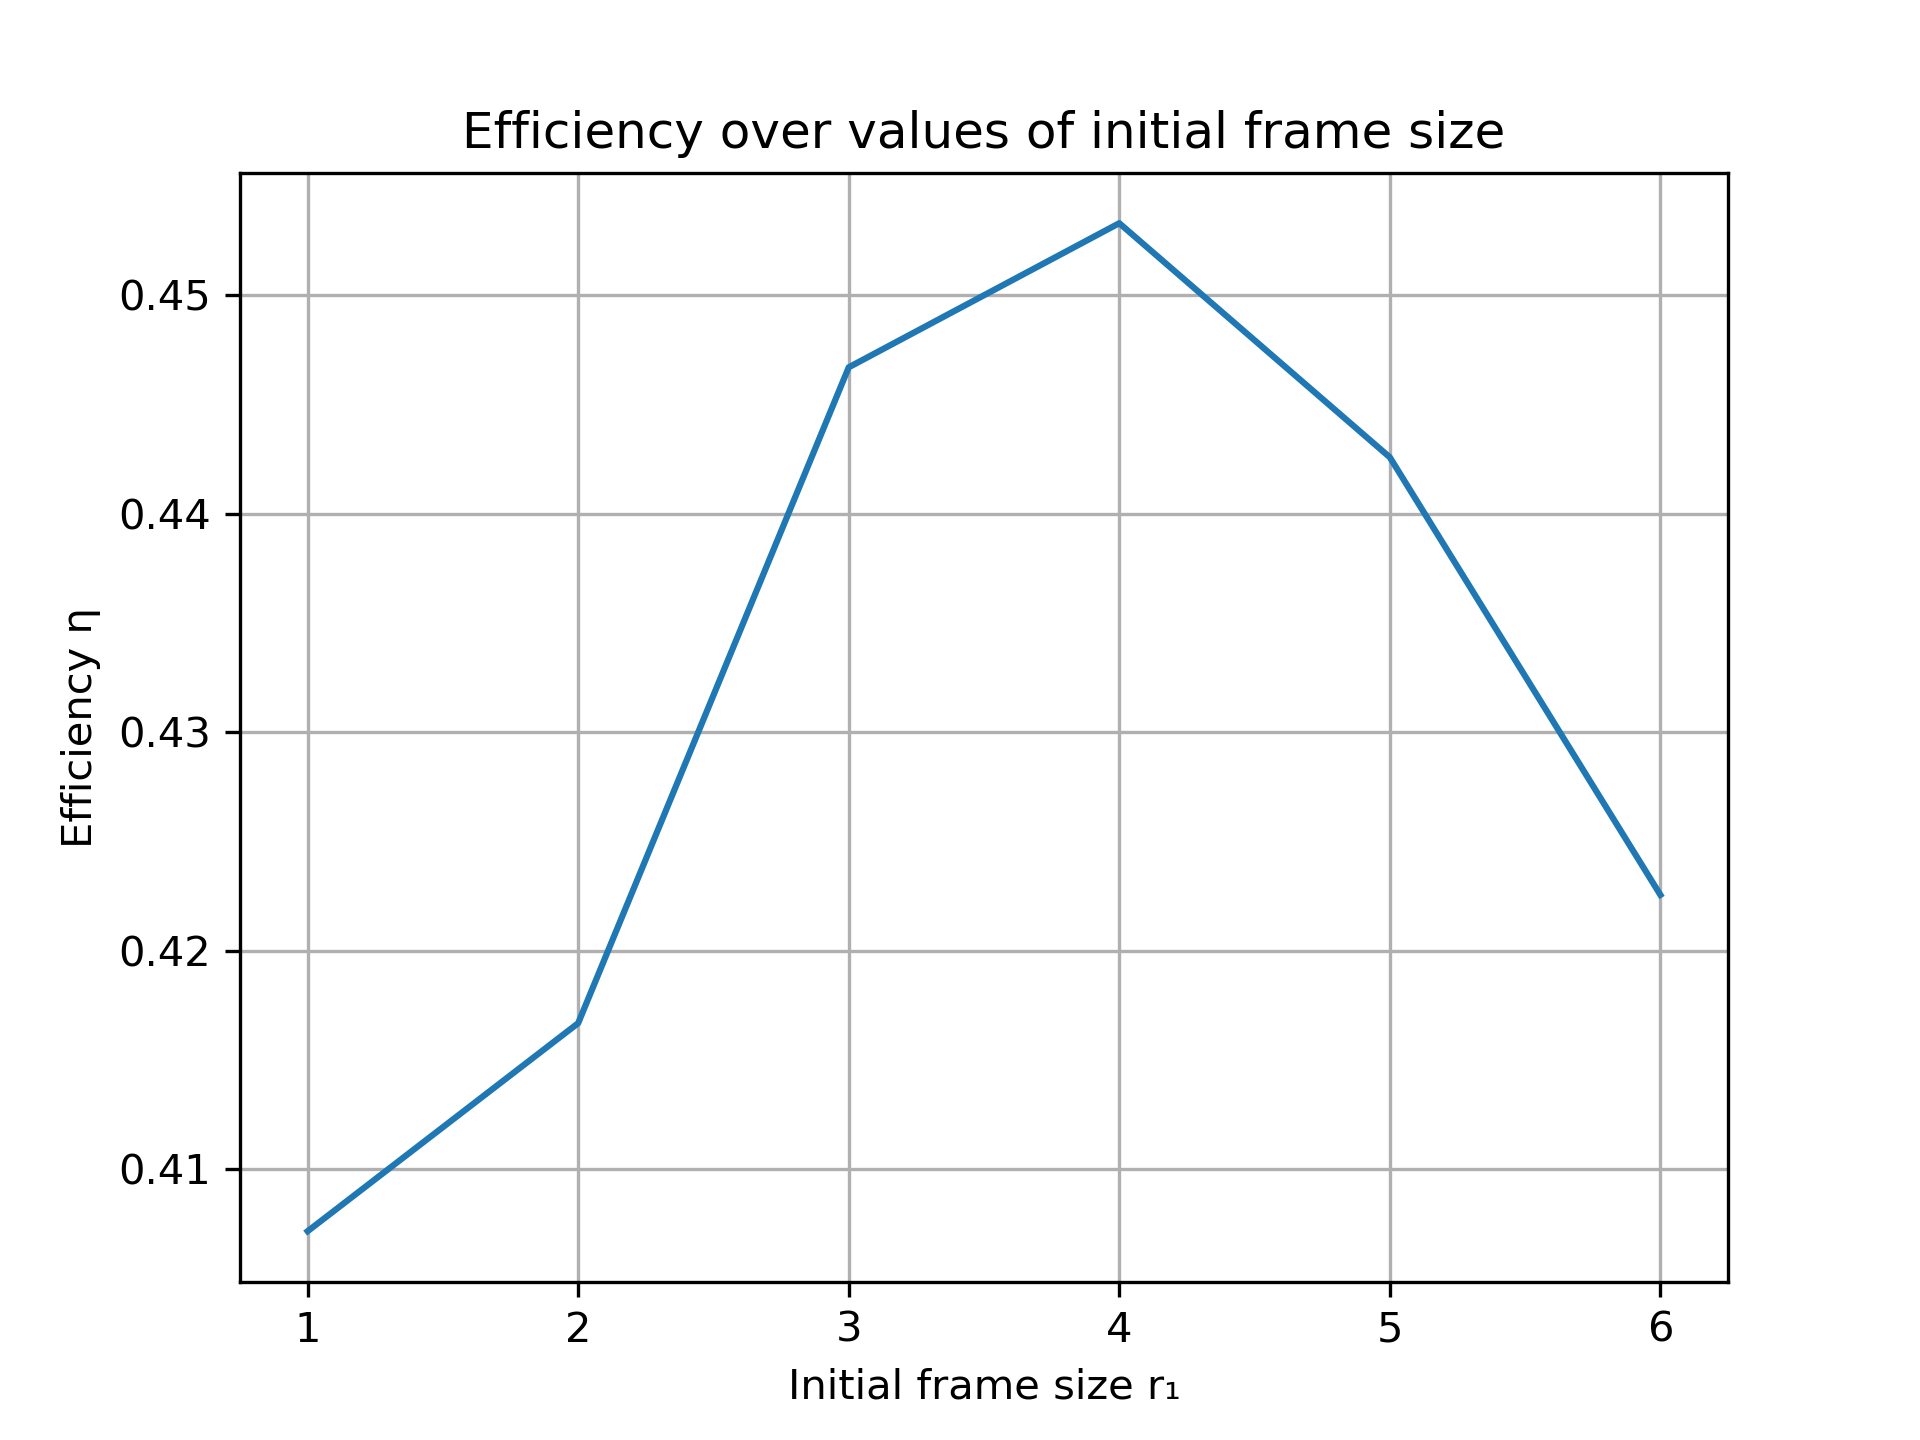
\includegraphics[width=15cm]{../res/hr-plot}
\end{center}

\section{Comment on expected efficiency behaviour of the system}

As anticipated by theory lectures, the case in which the \textsc{Dynamic Frame ALOHA}'s algorithm maximizes efficiency is the one in which the frame size ($r$) is dynamically updated to the current backlog (tags to solve at the next step, $n$).

\smallskip

Also, a direct consequence of the algotihm's behaviour will confirm the minimum being in $r = 1$.

\smallskip

$\Rightarrow max(\eta)$ is in $r = N$.

\smallskip

$\Rightarrow min(\eta)$ is in $r = 1$.

\subsection{Demonstration: efficiency maximum and minimum points in $r = 1$ and $r = N$}

Let $\eta = \dfrac{N}{r} \cdot \left(1 - \dfrac{1}{r}\right)^{N-1}$ be defined as the efficiency of the algorithm.

\medskip

As known from Mathematical Analisys, to highlight maximum points we will just need to null the derivative $\dfrac{d \eta}{d r}$.

\medskip

Note that, for the existance of the derivative, $r \neq 0$, which is trivially proved by the layout of slots and $N > 1$ being constant.

\medskip

$\dfrac{d \eta}{d r} = \dfrac{N \cdot \left(\dfrac{r-1}{r}\right)^{N+1} \cdot \left(r - N\right)}{\left(r - 1\right)^3} = 0$

\bigskip

Which, simplified, becomes:

\medskip

$\dfrac{N}{r^3} \cdot \left(\dfrac{r - 1}{r}\right)^{N-2} \cdot (-r + N) = 0$

\bigskip

And, when used to distinguish maximum points from minimum ones, translates to:

\medskip

$\dfrac{N}{r^3} \cdot \left(\dfrac{r - 1}{r}\right)^{N-2} \cdot (-r + N) \geq 0$ (with $r \neq 0$ from existance conditions).

\bigskip

Underlining the two cases:

\begin{equation*}
    \begin{cases}
        r-1 \geq 0\\
        -r+N \geq 0
    \end{cases}\,\Rightarrow
    \begin{cases}
        r \geq 1\\
        r \leq N
    \end{cases}\,
\end{equation*}

\medskip

In which $N$ is again trivially $> 1$.

\bigskip

This will ultimately yield to the final result:

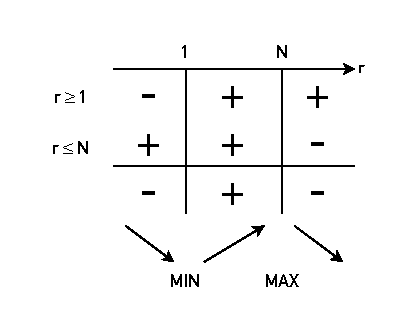
\includegraphics[width=8cm]{../res/efficiency-system-minmax}

\smallskip

Which confirms our expectations about the computed plot, underlining the minimum point being in $r = 1$ and the maximum one being in $r = N$.
\end{document}